\section{Úvod}
Následující dokument popisuje implementaci jazyka IFJ17. Jedná se o projekt,
který byl vyprácován posle zadání do předmětů IAL a IF na Fakultě
informačních technologiích Vysokého učení technického v Brně.
Dokumentace je logicky členěna na několik kapitoly.
\section{Teoretický rozbor zadání}
Naším úkolem bylo implementoval překladač z podmnožiny jazyka Free Basic
do mezikódu IFJcode17.

Jazyk není case-sensitive, což znamená že nerozlišuje malá a velká
písmena v názvech identifikátorů a klíčových slov.

Pro implementaci byl použit tzv. Syntaxí řízený překlad.
Implementaci překladače byla se nám tedy rozdělila na několik částí.
Lexikální analyzátor, syntaktický analyzátor, sémantický analyzátor,
generáto cílového kódu a optimalizátor kódu. Propojení jednotlivých
komponent naznačuje následující schéma.
\vspace*{16px}
\begin{figure}[htbp]
\centering
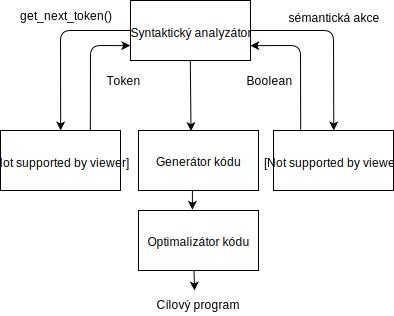
\includegraphics[width=0.7\textwidth, angle=0]{src/assets/structure.pdf}
\end{figure}

V následující části bude každá část interpretu posána podrobněji.